%小角正弦极限

\pentry{极限\upref{Lim}}

这里要介绍的是一个很显然的几何问题,然而它在高等数学和物理中却非常频繁地出现.

设平面上 $O$ 点为圆心,以 $R$ 作为半径画圆.取一段的圆心角为 $\theta $ 的圆弧 $AB$ (令长为 $l$),并作线段 $AB$ (如\autoref{LimArc_fig1}).

\begin{figure}[ht]
\centering
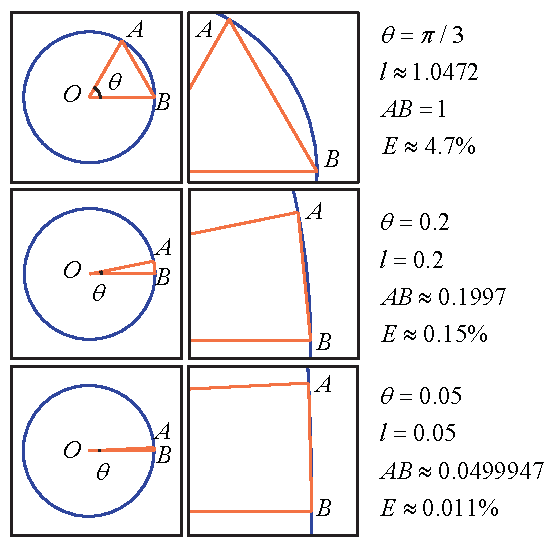
\includegraphics[width=10cm]{./figures/LimArc1.pdf}
\caption{单位圆中,随着角度不断减小,弧长与线段长度的相对误差也不断减小}\label{LimArc_fig1}
\end{figure}

由弧长公式得
\begin{equation} \label{LimArc_eq1}
l = R\theta 
\end{equation}
线段 $AB$ 的长度为
\begin{equation}\label{LimArc_eq2}
AB = 2R\sin \frac{\theta }{2}
\end{equation}
显然弧长 $l$ 大于线段长度$AB$ (两点之间直线最短),但从图中可以看出随着 $\theta $ 越来越小,二者的相对误差($E$)越来越小.用极限\upref{Lim}的语言来说,就是当 $\theta $ \bb{趋近于 $0$ } 时,它们的比值\bb{趋近于1}\footnote{注意这只是一个经验上的总结,证明参考高等数学教材.}.现在我们可以总结出 $\theta \to 0$ 时的两个结论

\begin{enumerate}
\item 线段长度 $AB$ 趋近于弧长 $l$, 一般情况下可近似认为 $AB = l$ \footnote{严格来说,这是一个一阶近似,见泰勒级数.}. % 链接未完成

\item 代入上面的长度表达式(\autoref{LimArc_eq1}),有
\begin{equation}
1=\lim_{\theta\to 0} \frac{AB}{l} = \lim_{\theta\to 0} \frac{2R\sin (\theta/2)}{R\theta} 
= \lim_{\theta\to 0}\frac{\sin (\theta/2)}{\theta/2}
\end{equation}
令 $x = \theta/2$, 有
\begin{equation}
\lim_{\theta\to 0} \frac{\sin x}{x} = 1
\end{equation}
\end{enumerate}

这是一个非常重要的极限.










